\documentclass[aspectratio=169,11pt]{beamer}
% ---------------------------------------------------------------------------
% Tema Beamer "archdati" — accento unico teal/indaco, font Lato, pdflatex.
% Colorato ma sobrio; niente slide divisorie vuote; footer con barra di
% avanzamento (per regolarsi sui tempi durante l'orale).
% ---------------------------------------------------------------------------
\usepackage[T1]{fontenc}
\usepackage[utf8]{inputenc}
\usepackage[italian]{babel}
\usepackage{csquotes}
\usepackage{lato}
\usepackage{inconsolata}
\renewcommand{\familydefault}{\sfdefault}
\usepackage{tikz}
\usepackage{pgfplots}
\pgfplotsset{compat=1.18}
\usepackage{booktabs}
\usepackage{colortbl}
\usepackage{array}

% --- Palette -----------------------------------------------------------------
\definecolor{teal}{HTML}{0E7C86}      % accento primario
\definecolor{ink}{HTML}{22314F}       % inchiostro (testo/titoli)
\definecolor{sfondo}{HTML}{FAF9F6}    % off-white caldo
\definecolor{amber}{HTML}{E0A458}     % highlight riservato (dato chiave / vincitore)
\definecolor{grigio}{HTML}{6B7280}
\definecolor{grigiochiaro}{HTML}{DED9D3}
\definecolor{pgblu}{HTML}{336791}     % identita' Citus/PostgreSQL
\definecolor{mongoverde}{HTML}{00684A}% identita' MongoDB

% --- Base --------------------------------------------------------------------
\usetheme{default}
\setbeamertemplate{navigation symbols}{}
\setbeamertemplate{blocks}[rounded][shadow=false]
\setbeamercolor{background canvas}{bg=sfondo}
\setbeamercolor{normal text}{fg=ink}
\setbeamercolor{structure}{fg=teal}
\setbeamercolor{frametitle}{fg=ink}
\setbeamercolor{itemize item}{fg=teal}
\setbeamercolor{itemize subitem}{fg=teal}
\setbeamercolor{enumerate item}{fg=teal}
\setbeamerfont{frametitle}{series=\bfseries,size=\Large}
\setbeamerfont{title}{series=\bfseries,size=\huge}
\usebeamercolor[fg]{normal text}

% --- Titolo di frame con riga d'accento --------------------------------------
\setbeamertemplate{frametitle}{%
  \vspace*{0.7em}%
  {\usebeamerfont{frametitle}\usebeamercolor[fg]{frametitle}\insertframetitle}\\[0.18em]%
  {\color{teal}\rule{2.4em}{2.4pt}}%
  \vspace*{0.1em}%
}

% --- Footer: sezione + n/tot + barra di avanzamento --------------------------
\setbeamertemplate{footline}{%
  \leavevmode%
  \hbox to \paperwidth{\hspace{1.4em}%
    {\footnotesize\color{grigio}\insertsection}\hfill
    {\footnotesize\color{grigio}\insertframenumber\,/\,\inserttotalframenumber}%
    \hspace{1.4em}}%
  \vskip3pt%
  \ifnum\inserttotalframenumber>0
    {\color{teal}\rule{\dimexpr\paperwidth*\insertframenumber/\inserttotalframenumber\relax}{2.2pt}}%
    {\color{grigiochiaro}\rule{\dimexpr\paperwidth-\paperwidth*\insertframenumber/\inserttotalframenumber\relax}{2.2pt}}%
  \else
    {\color{grigiochiaro}\rule{\paperwidth}{2.2pt}}%
  \fi
}

% --- Blocchi ----------------------------------------------------------------
% Blocco per uno dei due sistemi (colore identitario in intestazione).
\newenvironment{sysblock}[2]{%
  \setbeamercolor{block title}{bg=#1,fg=white}%
  \setbeamercolor{block body}{bg=#1!7,fg=ink}%
  \begin{block}{#2}}{\end{block}}

% Blocco "risultato / verdetto" con accento ambra.
\newenvironment{keyblock}[1]{%
  \setbeamercolor{block title}{bg=amber,fg=ink}%
  \setbeamercolor{block body}{bg=amber!12,fg=ink}%
  \begin{block}{#1}}{\end{block}}

% Evidenziazione inline del dato chiave.
\newcommand{\dato}[1]{{\color{teal}\bfseries #1}}
\newcommand{\vince}[1]{{\color{teal}\bfseries #1}}

% --- Codice (listings) ------------------------------------------------------
\usepackage{listings}
\lstset{
  basicstyle=\ttfamily\footnotesize,
  keywordstyle=\color{teal}\bfseries,
  commentstyle=\color{grigio}\itshape,
  stringstyle=\color{amber!80!black},
  backgroundcolor=\color{ink!6},
  frame=leftline, rulecolor=\color{teal}, framesep=6pt, xleftmargin=8pt,
  breaklines=true, showstringspaces=false, columns=fullflexible,
  captionpos=b, aboveskip=4pt, belowskip=2pt,
}

\graphicspath{{../report/figure/}}

\title{Progetto Architetture Dati - Confronto scalabilità tra DBMS relazionale e non relazionale}
\subtitle{Valutazione empirica della scalabilità in ambiente distribuito di PostgreSQL e MongoDB}
\author{Fabio Compagnoni}

\begin{document}

% ===== 1. Titolo ============================================================
{\setbeamertemplate{footline}{}
\begin{frame}[plain]
  \begin{tikzpicture}[remember picture,overlay]
    \fill[teal] (current page.north west) rectangle ([yshift=-3.6cm]current page.north east);
    \node[anchor=north west,text=white,font=\huge\bfseries,text width=0.88\paperwidth]
      at ([xshift=1.4em,yshift=-0.9cm]current page.north west)
      {Progetto Architetture Dati};
  \end{tikzpicture}
  \vspace{3.9cm}\par
  {\large\color{ink}\bfseries Confronto scalabilità tra DBMS relazionale e non relazionale}\\[0.2em]
  {\color{grigio}Dominio HR/retributivo multitenant}
  \vfill
  {\color{ink}\textbf{Fabio Compagnoni} — matricola 944954}\\[0.15em]
  {\footnotesize\color{grigio}Università degli Studi di Milano-Bicocca}
\end{frame}}

% ===== 2. Progetto e obiettivo =============================================
\section{Progetto}
\begin{frame}{Il progetto e l'obiettivo}
  Da un \textbf{caso reale} (buste paga in formato XML) si sono progettati \textbf{due schemi sui medesimi dati}:
  \begin{itemize}
    \item un database \textbf{relazionale} distribuito — \textbf{PostgreSQL + Citus};
    \item un database \textbf{non relazionale} distribuito — \textbf{MongoDB}.
  \end{itemize}
  \vspace{0.3em}
  \begin{keyblock}{La domanda}
    A parità di dominio e di dati, \dato{quale dei due modelli scala meglio e ha performance migliori?}
  \end{keyblock}
  \vspace{0.2em}
  Due filosofie opposte, stessa classe CAP (entrambi \textbf{CP}): normalizzazione e \emph{join} da un lato,
  aggregato ed \emph{embedding} dall'altro.
\end{frame}

% ===== 3. Dominio ===========================================================
\begin{frame}{Il dominio: HR e retribuzioni}
  \begin{itemize}
    \item Gestione del personale e delle \textbf{paghe}: \textbf{più aziende clienti} sullo stesso sistema
          (regime \textbf{multitenant}).
    \item Origine \textbf{reale} (XML di cedolini); per il GDPR il dataset è \textbf{sintetico ma calibrato},
          riproducibile (seed). Base: 30 ditte / 554 dip.\ $\rightarrow$ migliaia di ditte.
    \item Il \textbf{cedolino} è l'aggregato centrale, ma poggia su una struttura relazionale profonda
          (anagrafiche, cataloghi condivisi).
  \end{itemize}
  \vspace{0.3em}
  \begin{keyblock}{Perché il \texttt{tenant\_id} (la ditta) è centrale}
    È la \textbf{chiave di partizionamento}: \dato{distribuisce i dati sui nodi} in \textbf{entrambi} i sistemi, tenendo \textbf{co-locati} i dati di un'azienda su un solo nodo (una ditta $=$ un nodo). \textbf{Ma è anche un limite}: se quel nodo cade, \dato{tutte le query di quell'azienda falliscono}, come confermato dai test sui guasti.
  \end{keyblock}
\end{frame}

% ===== 4. Teorema CAP ======================================================
\section{Modellazione}
\begin{frame}{Il teorema CAP: perché due sistemi CP}
  \begin{columns}[c]
    \begin{column}{0.44\textwidth}
      \centering
      \resizebox{\linewidth}{!}{%
      \begin{tikzpicture}[font=\footnotesize]
        \coordinate (A) at (0,2.6);
        \coordinate (C) at (-2.25,-1.3);
        \coordinate (P) at (2.25,-1.3);
        \draw[grigio,thick] (A)--(C);
        \draw[grigio,thick] (A)--(P);
        \draw[amber,line width=1.8pt] (C)--(P);
        \node[above=3pt] at (A) {\textbf{A}\; Disponibilità};
        \node[below left=0pt] at (C) {\textbf{C}\; Consistenza};
        \node[below right=0pt] at (P) {\textbf{P}\; Partizioni};
        \node[grigio] at (-0.78,0.58) {CA};
        \node[grigio] at (0.78,0.58) {AP};
        \node[ink] at (0,-0.72) {\textbf{CP}};
        \node[grigio,anchor=west] at (1.75,0.35) {Cassandra};
        \node[teal,align=center,font=\bfseries] at (0,-2.15) {PostgreSQL\\MongoDB};
      \end{tikzpicture}}
    \end{column}
    \begin{column}{0.56\textwidth}
      Di fronte a un \textbf{partizionamento di rete}, un sistema distribuito può garantire solo \textbf{2 proprietà su 3}: Consistenza, Disponibilità, Partition tolerance.
      \vspace{0.5em}

      Le partizioni \textbf{accadono}: la scelta reale è tra \textbf{CP} e \textbf{AP}. In un dominio \textbf{retributivo} la \dato{consistenza è irrinunciabile} (nessun cedolino incoerente), quindi entrambi i sistemi scelti sono \textbf{CP}.
      \vspace{0.5em}

      \textbf{Cassandra}, ad esempio, è un sistema \textbf{AP}: in caso di partizione privilegia la disponibilità a scapito della consistenza, quindi non è adatta a un dominio retributivo.
    \end{column}
  \end{columns}
\end{frame}

% ===== 5. Scelta dei due DBMS ==============================================
\begin{frame}{La scelta dei due DBMS}
  \small
  Entrambi \textbf{CP}, ma scelti per ragioni distinte, uno per ciascun modello di dato:
  \vspace{0.5em}
  \begin{columns}[T]
    \begin{column}{0.5\textwidth}
      \begin{sysblock}{pgblu}{Relazionale: PostgreSQL + Citus}
        PostgreSQL non è distribuito di default: lo si è reso tale con l'estensione \textbf{Citus} (coordinator e worker), che espone primitive di distribuzione \textbf{esplicite} (tabelle distribuite, reference
        table, co-locazione) mantenendo SQL completo, transazioni distribuite (2PC) e integrità referenziale.
      \end{sysblock}
    \end{column}
    \begin{column}{0.5\textwidth}
      \begin{sysblock}{mongoverde}{NoSQL: perché proprio MongoDB}
        Tra le \textbf{molte famiglie NoSQL} (chiave-valore, wide-column, grafo, documentale) è il
        \textbf{dominio} a decidere: il cedolino è un \textbf{aggregato}, quindi modello \textbf{documentale}.
        Tra i documentali, MongoDB unisce maturità e aggregation framework a \dato{transazioni multi-documento
        ACID stabili}, non scontate nel mondo NoSQL e richieste dal progetto.
      \end{sysblock}
    \end{column}
  \end{columns}
\end{frame}

% ===== 5. Schema ER completo (relazionale) =================================
\begin{frame}{Schema ER completo}
  \centering
  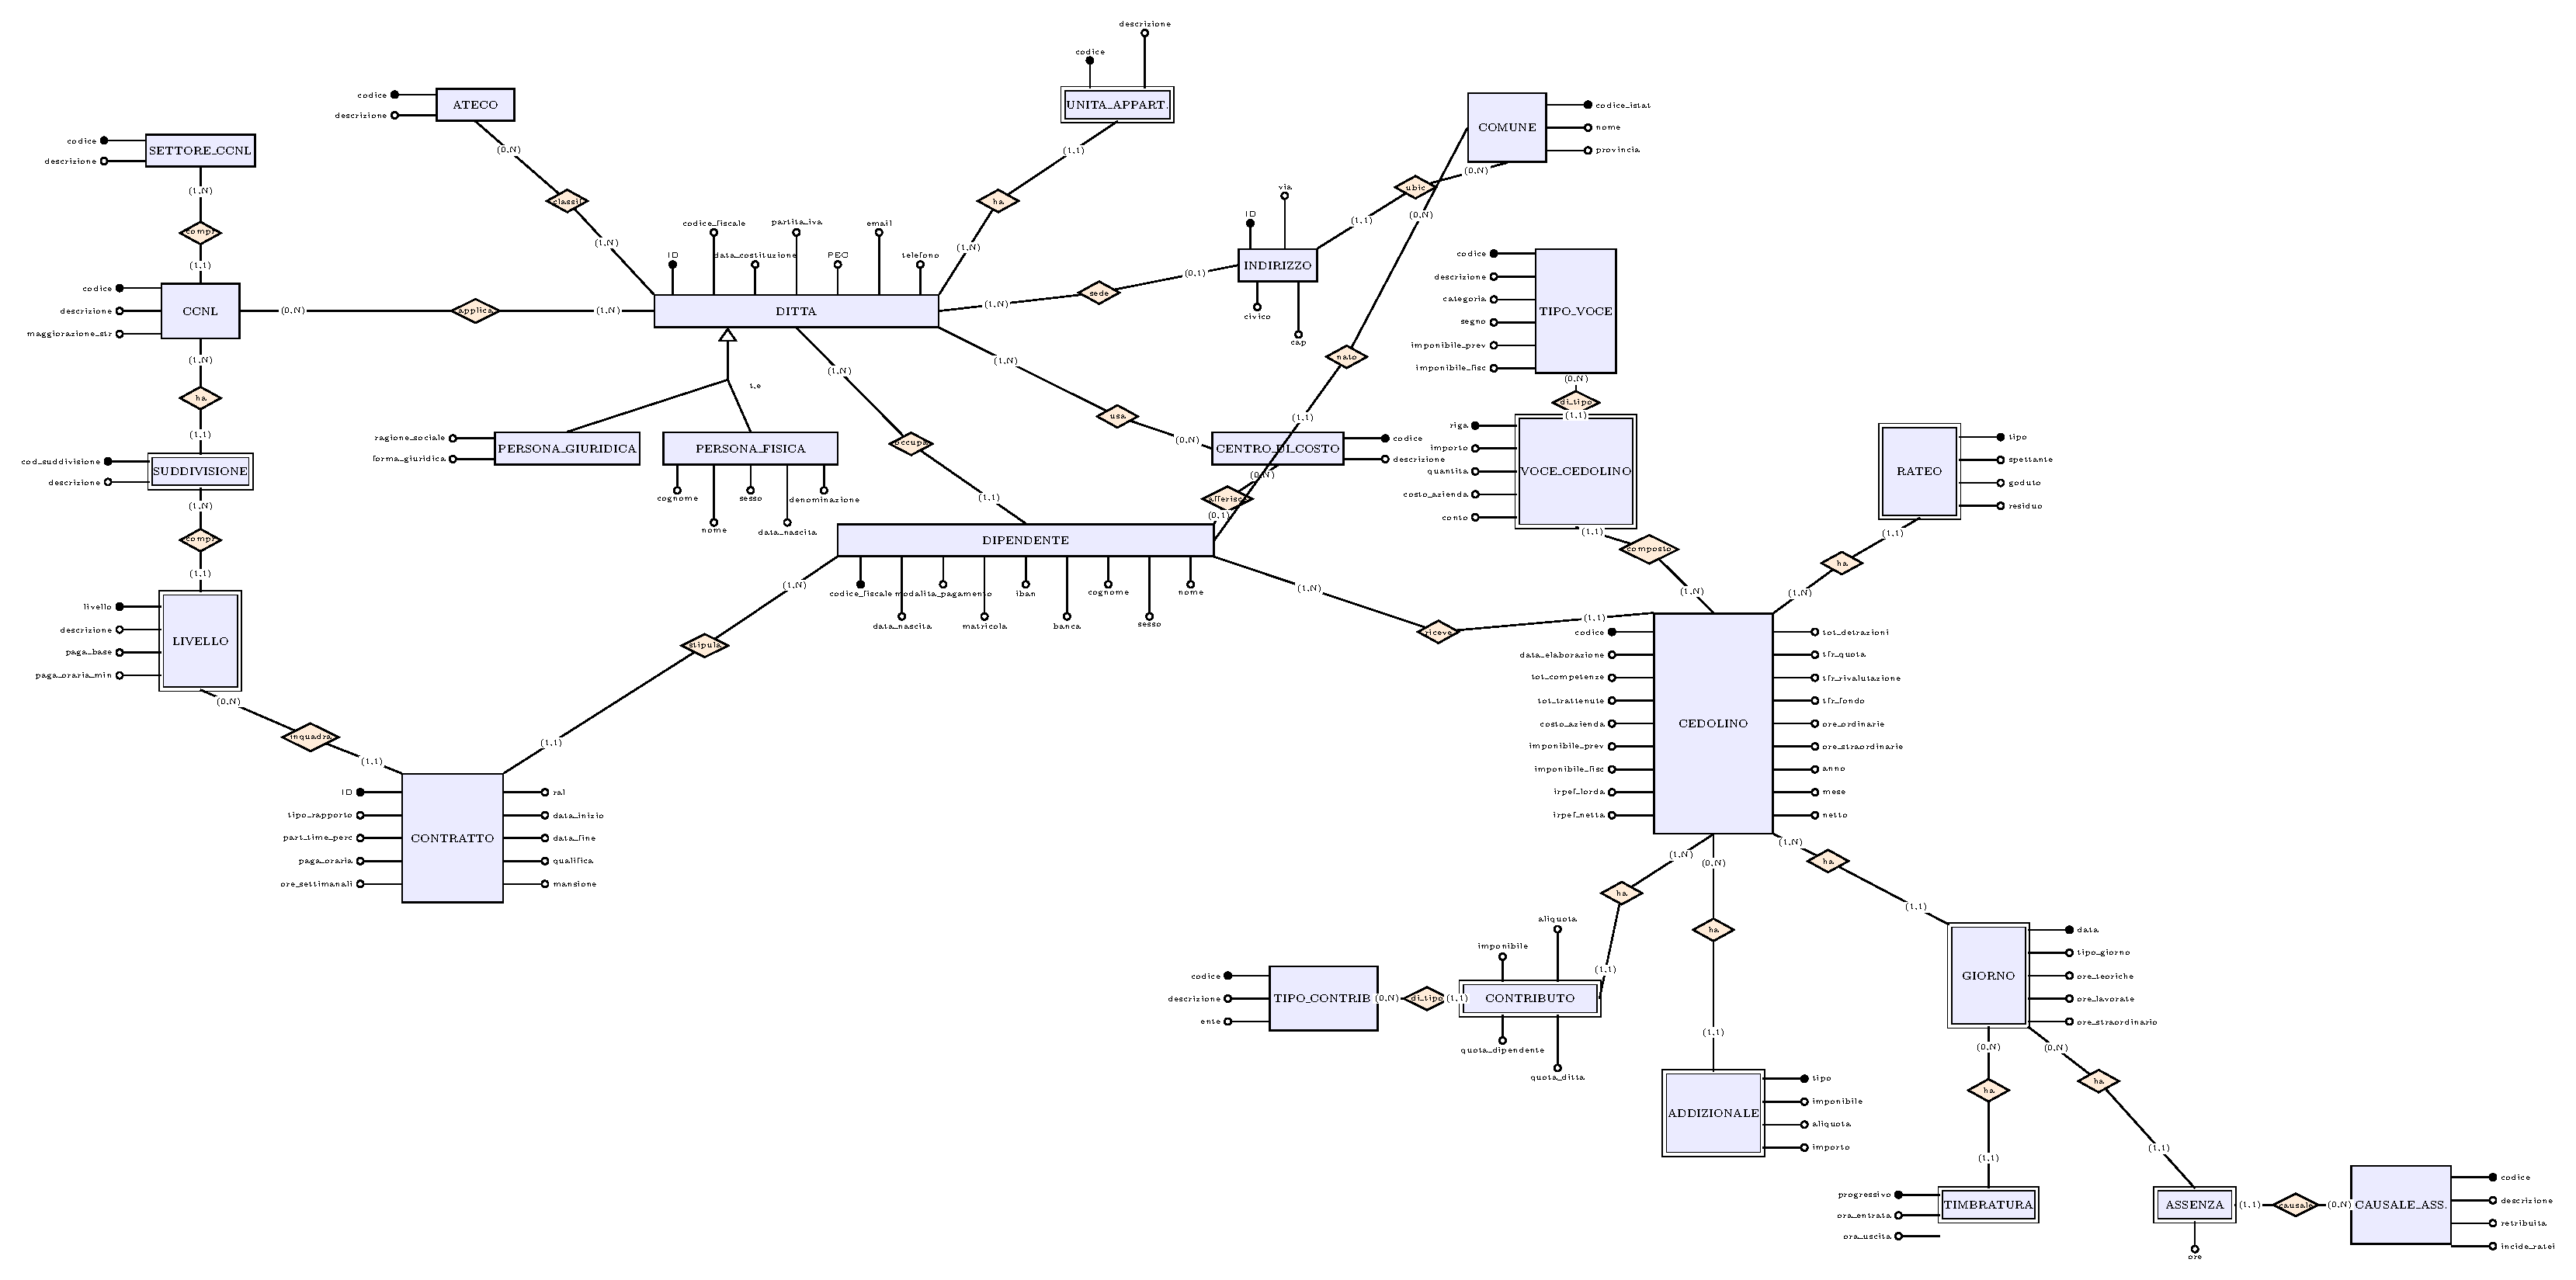
\includegraphics[width=\linewidth,height=6.1cm,keepaspectratio]{er-completo}
\end{frame}

% ===== 6. Schema documentale (MongoDB) =====================================
\begin{frame}[fragile]{Schema documentale: la collezione \texttt{cedolini}}
  \small Nel modello documentale il cedolino è \dato{un unico documento}: l'anagrafica è uno \emph{snapshot} embedded e voci, ratei, contributi e addizionali sono \textbf{array annidati}. 
  Si legge e si scrive con una sola operazione, senza join.
  \vspace{0.1em}
  \begin{lstlisting}[basicstyle=\ttfamily\scriptsize,aboveskip=2pt,belowskip=2pt]
db.createCollection("cedolini", {
  validator: { $jsonSchema: {
    bsonType: "object",
    required: ["tenant_id","cedolino_id","dipendente_id","anno","mese",
               "dipendente","totali","voci"],
    properties: {
      tenant_id:{bsonType:"long"}, cedolino_id:{bsonType:"long"},
      dipendente_id:{bsonType:"long"}, anno:{bsonType:"int"},
      mese:{bsonType:"int", minimum:1, maximum:12},
      dipendente: {bsonType:"object"},   // snapshot anagrafico (embedded)
      totali:{bsonType:"object"}, voci:{bsonType:"array"},
      ratei:{bsonType:"array"}, contributi:{bsonType:"array"},
      addizionali:{bsonType:"array"}, giorni:{bsonType:"array"}
    }
}}});
  \end{lstlisting}
\end{frame}

% ===== 6. Distribuzione dei dati ===========================================
\begin{frame}[fragile]{Come si distribuiscono i dati}
  \small
  Su entrambi la chiave è \texttt{tenant\_id}; cambia il \emph{modo} in cui la distribuzione viene gestita.
  \begin{columns}[c]
    \begin{column}{0.38\textwidth}
      \centering
      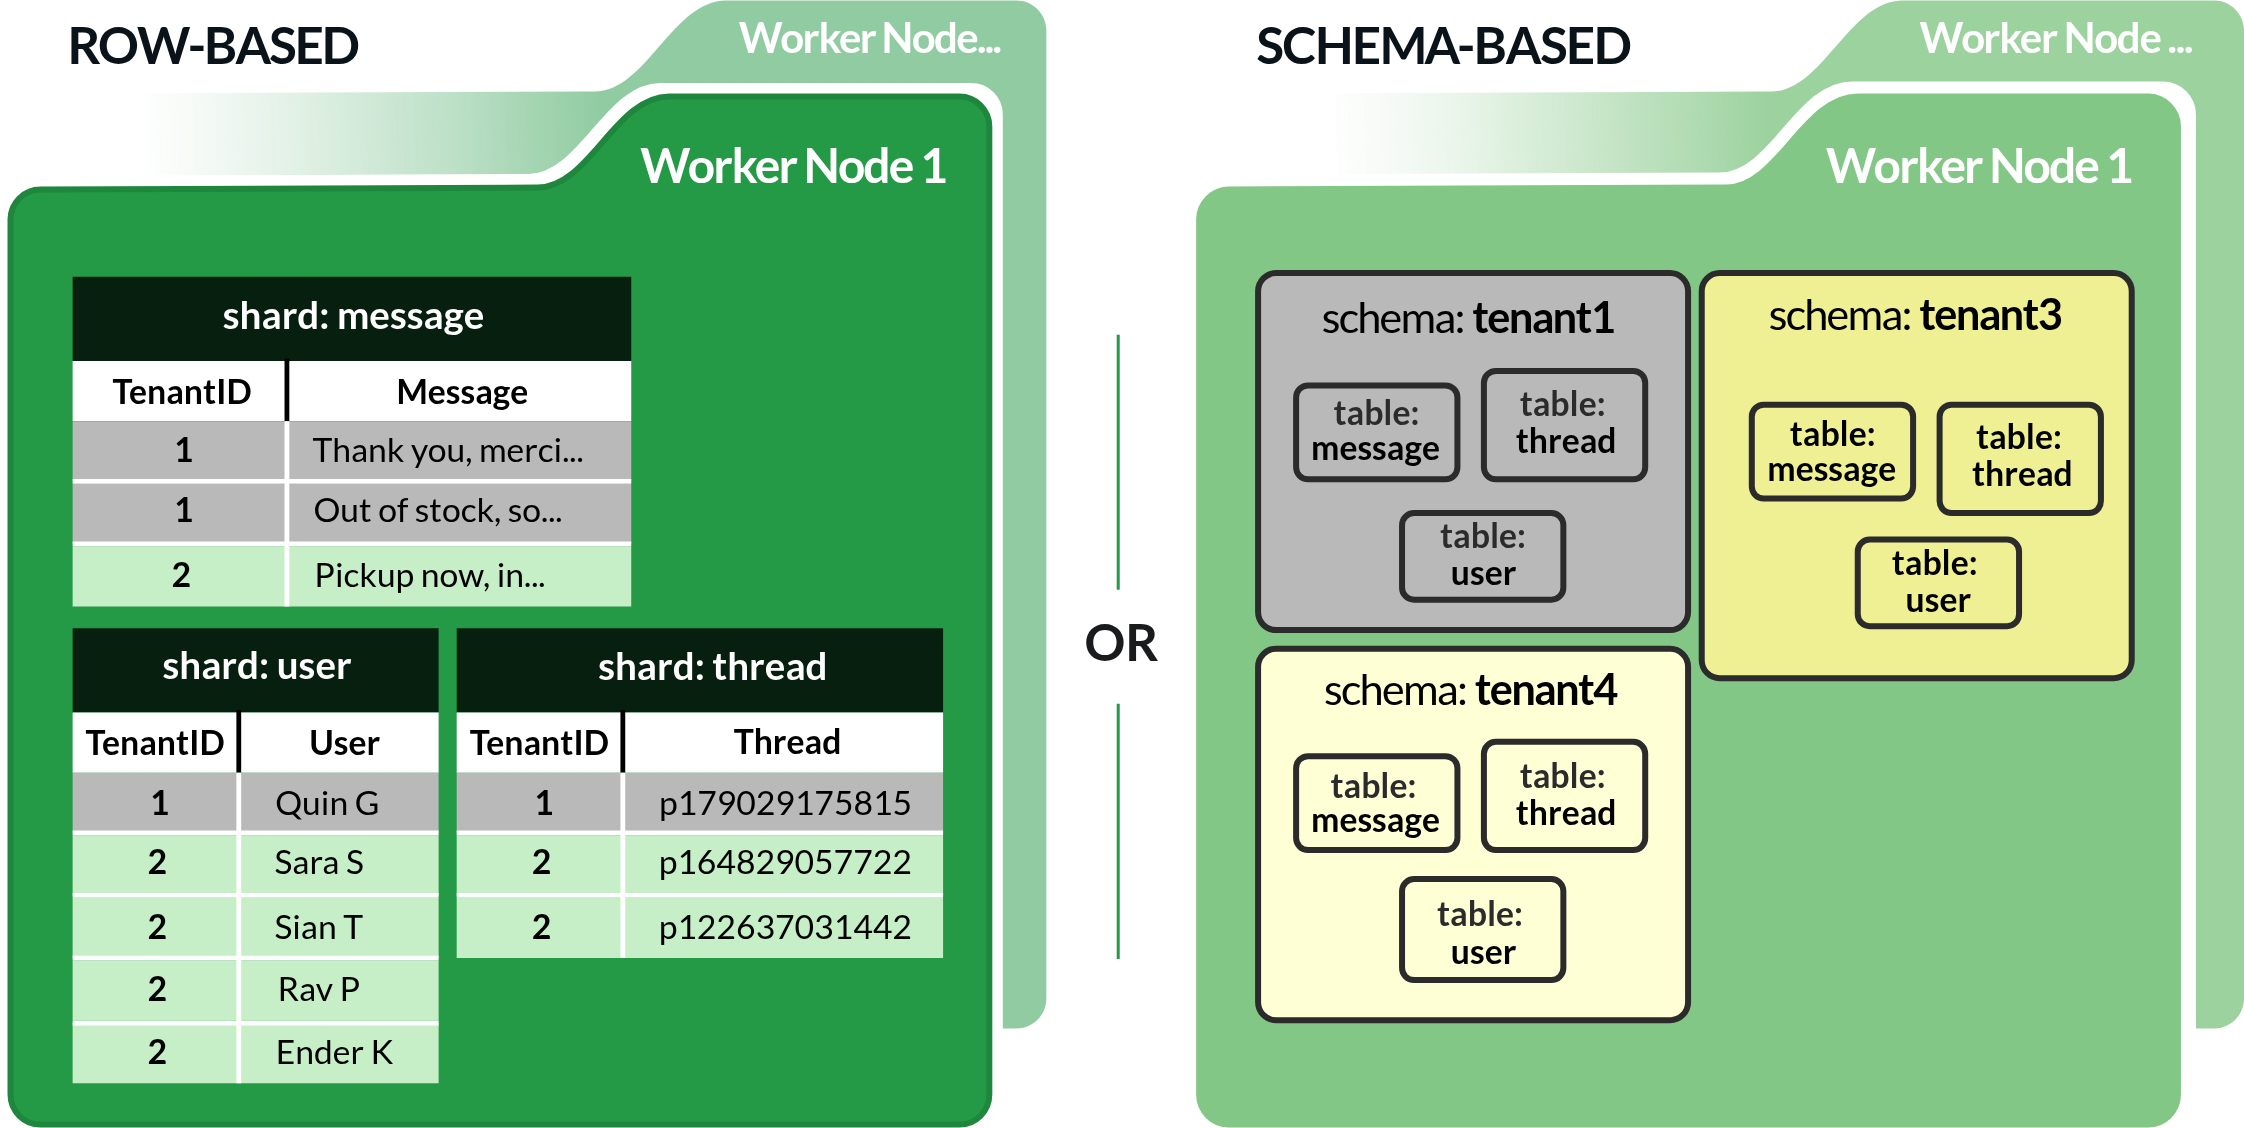
\includegraphics[width=\linewidth]{getting-started-two-ways-to-shard}\\[0.3em]
      {\scriptsize\color{grigio}Citus: \textbf{row-based} (scelto) vs schema-based}
    \end{column}
    \begin{column}{0.62\textwidth}
      \begin{sysblock}{pgblu}{Citus: distribuzione esplicita}
        \textbf{Row-based} per \texttt{tenant\_id}; cataloghi \textbf{reference table}; tabelle di un tenant \textbf{co-locate} su un solo shard. Rebalance \dato{manuale}, via \textbf{script dedicato}.
      \end{sysblock}
      \begin{sysblock}{mongoverde}{MongoDB: distribuzione automatica}
        \textbf{Sharded cluster} (l'altra opzione era il \textbf{replica set}): shard key \texttt{tenant\_id}, dati in
        \textbf{chunk} ridistribuiti da un \textbf{balancer} oltre una soglia (3$\times$ la range size).
        \dato{Nei test si è ridotta la range size} per distribuire su tutti gli shard.
      \end{sysblock}
    \end{column}
  \end{columns}
  \begin{lstlisting}[language=SQL,basicstyle=\ttfamily\scriptsize,aboveskip=2pt,belowskip=0pt]
SELECT citus_add_node('10.0.1.5', 5432);                                -- sul coordinator
SELECT rebalance_table_shards(shard_transfer_mode := 'block_writes');
  \end{lstlisting}
\end{frame}

% ===== 7. Metodologia =======================================================
\section{Metodologia}
\begin{frame}{Infrastruttura utilizzata per i test}
  \small Le misure sono state fatte su un cluster reale in cloud strutturato da una VM più potente che è stata utilizzata come coordinator ed entry point, e da quattro nodi-dati con le stesse caratteristiche hardware in modo da ottenere una scaling equo tra i nodi.
  \vspace{0.4em}
  \centering
  \footnotesize
  \renewcommand{\arraystretch}{1.3}
  \begin{tabular}{@{}llccl@{}}
    \toprule
    \textbf{Ruolo} & \textbf{VM (IP privato)} & \textbf{vCPU} & \textbf{RAM} & \textbf{Funzione} \\
    \midrule
    Coordinator & worker-1 (10.0.1.8) & 16 & 32\,GB & Citus coordinator / Mongo config+mongos \\
    Nodo-dati   & VM-1 (10.0.1.4)     & 4  & 16\,GB & worker / shard \\
    Nodo-dati   & VM-2 (10.0.1.5)     & 4  & 16\,GB & worker / shard \\
    Nodo-dati   & VM-3 (10.0.1.7)     & 4  & 16\,GB & worker / shard \\
    Nodo-dati   & VM-4 (10.0.1.6)     & 4  & 16\,GB & worker / shard \\
    \bottomrule
  \end{tabular}
  \vspace{0.4em}
  Ogni nodo ha un disco da 30 GB.
\end{frame}

% ===== 8. Generazione del dataset ==========================================
\begin{frame}[fragile]{Script di generazione dei dati: \texttt{genera.py}}
  \small Script \textbf{Python} parametrico e \textbf{riproducibile}: stesso comando $\Rightarrow$ stesso dataset.
  \vspace{0.3em}
  \begin{columns}[T]
    \begin{column}{0.55\textwidth}
      \textbf{Come sono generati i dati}
      \begin{itemize}\setlength\itemsep{2pt}
        \item \textbf{Fonti ufficiali}: comuni con \textbf{codice catastale} (Belfiore), codici \textbf{ATECO}, \textbf{CCNL} e settori (export \textbf{CNEL}).
        \item \textbf{Dai cedolini reali} (Centropaghe): tipi voce, tipi contributo, causali di assenza.
        \item \textbf{Sintetici} (GDPR): ditte, dipendenti, cedolini; il \dato{codice fiscale} è calcolato con l'algoritmo reale.
      \end{itemize}
    \end{column}
    \begin{column}{0.45\textwidth}
      \textbf{Due formati, dagli stessi dati}
      \begin{itemize}\setlength\itemsep{2pt}
        \item \texttt{COPY} (\texttt{.sql}) $\rightarrow$ Citus
        \item \texttt{JSONL} $\rightarrow$ \texttt{mongoimport}
      \end{itemize}
      \vspace{0.3em}
      \textbf{Caricamento} nei DB con gli script \texttt{carica-citus.sh} / \texttt{carica-mongo.sh}.
    \end{column}
  \end{columns}
  \vspace{0.2em}
  \begin{lstlisting}[basicstyle=\ttfamily\scriptsize,aboveskip=2pt,belowskip=0pt]
python3 data/genera.py --tenant-count 30 --dip-min 10 --dip-max 25 --seed 42 --out generato
bash scripts/carica-citus.sh generato/citus      # oppure: carica-mongo.sh generato/mongo
  \end{lstlisting}
\end{frame}

% ===== 8. Metodologia di test ==============================================
\begin{frame}{Metodologia di test}
  \small
  \begin{itemize}\setlength\itemsep{5pt}
    \item \textbf{Dati}: lo \dato{stesso dataset sintetico} sui due sistemi (seed fisso, riproducibile,
          calibrato sui cedolini reali), caricato in \textbf{bulk} (\texttt{COPY} / \texttt{mongoimport}) e
          cresciuto \textbf{a lotti}; suite speculare di 13 letture (dalle \dato{single-shard} alle
          \dato{cross-shard}) e 7 scritture.
    \item \textbf{Esecuzione}: \dato{una query alla volta} sotto carico sostenuto, con \texttt{pgbench} (Citus)
          e un loop \texttt{mongosh} (Mongo); letture a \textbf{parametri randomizzati}, scritture a
          \textbf{tenant fisso}; cache \textbf{fredda} (scaling nodi) o \textbf{calda} (scaling dati).
    \item \textbf{Raccolta e analisi}: contatori nativi per-nodo con \dato{azzera\,$\to$\,run\,$\to$\,delta}
          (\texttt{pg\_stat\_statements} via \texttt{run\_command\_on\_all\_nodes}, \texttt{serverStatus},
          \texttt{docker stats}, \texttt{/proc}). Ripetizioni \textbf{per tipo di test}: letture \dato{media su
          3 run}, scritture \dato{una sola esecuzione}, guasti \dato{10 run} (ogni volta con un nodo random spento). I CSV diventano poi tabelle e grafici.
  \end{itemize}
\end{frame}



% ===== 9. Script per ogni test =============================================
\begin{frame}{Gli script, per ogni tipo di test}
  \small Ogni esperimento è automatizzato da script dedicati, \textbf{speculari} tra i due sistemi.
  \vspace{0.4em}
  \centering
  \scriptsize
  \renewcommand{\arraystretch}{1.2}
  \begin{tabular}{@{}p{2.6cm} p{4.7cm} p{4.4cm}@{}}
    \toprule
    \textbf{Esperimento} & \textbf{PostgreSQL + Citus} & \textbf{MongoDB} \\
    \midrule
    Caricamento dati & \texttt{carica-citus.sh} (COPY) & \texttt{carica-mongo.sh} (mongoimport) \\
    Suite letture    & \texttt{esegui-suite-citus.sh}  & \texttt{esegui-suite-mongo.sh} \\
    Scaling per nodi & \texttt{citus-add-node.sh}\newline\texttt{citus-rebalance.sh} & \texttt{scala-nodi-mongo.sh} \\
    Scaling per dati & \texttt{scala-dati-citus.sh}    & \texttt{scala-dati-mongo.sh} \\
    Scritture        & \texttt{esegui-scritture-citus.sh} & \texttt{esegui-scritture-mongo.sh} \\
    Guasti           & \texttt{test-guasto-citus.sh}   & \texttt{test-guasto-mongo.sh} \\
    Cache / media    & \texttt{azzera-cache-citus.sh}\newline\texttt{media-citus.sh} & \texttt{azzera-cache-mongo.sh}\newline\texttt{media-mongo.sh} \\
    \bottomrule
  \end{tabular}
  \vspace{0.5em}
  \par I CSV raccolti diventano poi i grafici del capitolo risultati (\texttt{grafici.py}, matplotlib).
\end{frame}

% ===== 6. Scalabilità per nodi: Citus ======================================
\section{Risultati}
\begin{frame}{Scalabilità sui nodi: PostgreSQL + Citus}
  \begin{columns}[c]
    \begin{column}{0.5\textwidth}
      \small A parità di dati si passa da \textbf{1 a 4 nodi}, con \textbf{rebalance esplicito} a ogni passo.
      \begin{itemize}\setlength\itemsep{3pt}
        \item Le analitiche \textbf{cross-shard} scalano \dato{quasi linearmente}: speedup \dato{3.8--4.6$\times$} con 4 nodi (L04 72$\to$18\,ms, L11 76$\to$20\,ms).
        \item Le \textbf{single-shard} restano piatte (${\sim}$1.5\,ms): colpiscono un solo shard.
        \item Il lavoro \emph{per worker} (CPU, righe elaborate) cala coi nodi.
      \end{itemize}
    \end{column}
    \begin{column}{0.5\textwidth}
      \centering
      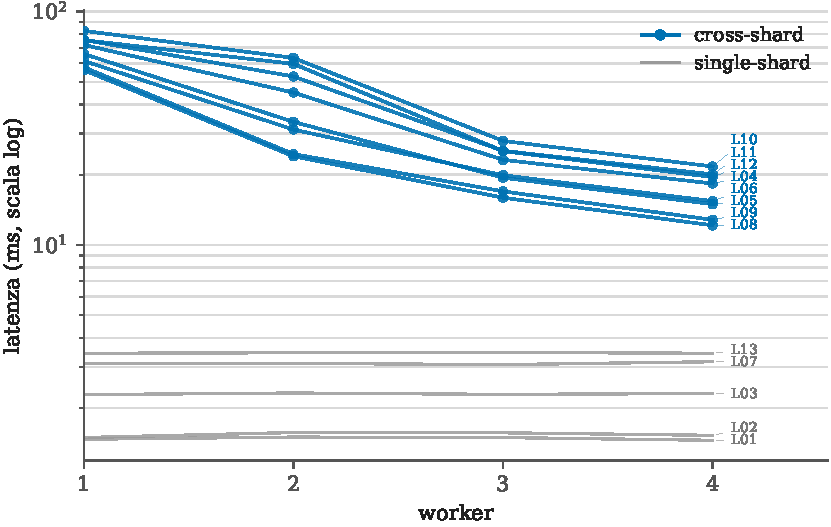
\includegraphics[width=\linewidth]{fig-scaling-nodi-citus}
    \end{column}
  \end{columns}
\end{frame}

% ===== 7. Scalabilità per nodi: MongoDB ====================================
\begin{frame}{Scalabilità sui nodi: MongoDB}
  \begin{columns}[c]
    \begin{column}{0.56\textwidth}
      \small A parità di dati si aggiungono shard, ma \dato{il balancer non distribuisce a questa scala}: la collezione \texttt{cedolini} (${\sim}$42\,MB) resta su un solo shard, perché la soglia di migrazione (3$\times$ la range size, cioè 384\,MB) non è mai raggiunta. 
      Anche riducendo la range size e splittando i chunk a mano, in \textbf{888 round} il balancer \textbf{non migra} i chunk sui nodi.
      \vspace{0.3em}
      \begin{keyblock}{Conseguenza}
        A 1 e 2 shard la latenza è \dato{identica} (L04 7$\to$7\,ms, L11 12$\to$12\,ms): aggiungere shard \textbf{non porta beneficio}. Mongo resta però più \textbf{veloce in assoluto}.
      \end{keyblock}
    \end{column}
    \begin{column}{0.44\textwidth}
      \centering
      \begin{tikzpicture}
      \begin{axis}[ybar,width=\linewidth,height=4.6cm,ylabel={CPU (\%)},
        symbolic x coords={shard 1,shard 2},xtick=data,ymin=0,ymax=44,
        nodes near coords,every node near coord/.append style={font=\scriptsize},
        bar width=22pt,tick label style={font=\small},label style={font=\footnotesize},
        enlarge x limits=0.5,ytick={0,10,20,30,40}]
        \addplot[fill=mongoverde,draw=mongoverde!70!black] coordinates {(shard 1,37.6) (shard 2,0.2)};
      \end{axis}
      \end{tikzpicture}\\
      {\scriptsize\color{grigio}CPU per shard sotto carico (2 shard): il 2\textsuperscript{o} resta inattivo}
    \end{column}
  \end{columns}
\end{frame}

% ===== 8. Scalabilità per nodi: confronto ==================================
\begin{frame}{Scalabilità sui nodi: confronto in sintesi}
  \centering
  \begin{tikzpicture}
  \begin{axis}[width=0.66\linewidth,height=5.1cm,xlabel={nodi / shard},ylabel={speedup ($\times$)},
    xtick={1,2,3,4},ymin=0,ymax=4.4,legend pos=north west,
    legend style={font=\small,draw=none,fill=none},
    tick label style={font=\small},label style={font=\small},
    grid=major,major grid style={grigiochiaro}]
    \addplot[dashed,grigio,thick] coordinates {(1,1)(4,4)};
    \addplot[teal,very thick,mark=*] coordinates {(1,1)(2,1.6)(3,3.1)(4,3.9)};
    \addplot[mongoverde,very thick,mark=square*] coordinates {(1,1)(2,1)(3,1)(4,1)};
    \legend{ideale,Citus,MongoDB}
  \end{axis}
  \end{tikzpicture}
  \par\vspace{0.4em}
  {\small Speedup su L04, cioè la latenza a 1 nodo divisa per quella a $n$ nodi. Citus si avvicina allo scaling
  \dato{ideale} (${\sim}4\times$ con 4 nodi), mentre MongoDB resta a \textbf{1$\times$}: a questa scala il balancer
  non ridistribuisce i dati.}
\end{frame}

% ===== Scalabilità per nodi: tabella completa ==============================
\begin{frame}{Scalabilità sui nodi: tutte le query in lettura (1--4 nodi)}
  \centering
  \scriptsize
  \renewcommand{\arraystretch}{1.0}
  \setlength{\tabcolsep}{4.5pt}
  \begin{tabular}{@{}l rrrr c rrr@{}}
    \toprule
    & \multicolumn{4}{c}{\textbf{Citus} (nodi)} & \textbf{sp.} & \multicolumn{3}{c}{\textbf{MongoDB} (shard)} \\
    \cmidrule(lr){2-5}\cmidrule(lr){7-9}
    \textbf{Query --- latenza (ms)} & \textbf{1} & \textbf{2} & \textbf{3} & \textbf{4} & 1$\to$4 & \textbf{1} & \textbf{2} & \textbf{3} \\
    \midrule
    L01 cedolino singolo    & 1.5 & 1.5 & 1.5 & 1.5 & 1.0$\times$ & 2.3 & 2.3 & 2.3 \\
    L02 cedolini ditta      & 1.5 & 1.6 & 1.6 & 1.5 & 1.0$\times$ & 2.7 & 2.7 & 2.7 \\
    L03 costo per centro    & 2.3 & 2.3 & 2.3 & 2.3 & 1.0$\times$ & 3.1 & 3.1 & 3.1 \\
    L04 gender gap mediano  & 71.9 & 45.0 & 23.2 & 18.3 & \dato{3.9$\times$} & 7.2 & 7.2 & 7.1 \\
    L05 top-N retribuzioni  & 65.8 & 33.7 & 19.4 & 14.9 & \dato{4.4$\times$} & 3.7 & 3.7 & 3.7 \\
    L06 assenteismo/mese    & 61.4 & 31.2 & 19.9 & 15.4 & \dato{4.0$\times$} & 100 & 99.5 & 99.9 \\
    L07 straordinari/centro & 3.1 & 3.1 & 3.1 & 3.2 & 1.0$\times$ & 2.9 & 2.9 & 2.9 \\
    L08 trend costo lavoro  & 56.1 & 24.0 & 15.9 & 12.1 & \dato{4.6$\times$} & 13.7 & 10.3 & 10.3 \\
    L09 organico/livello    & 57.7 & 24.5 & 17.0 & 12.8 & \dato{4.5$\times$} & 6.5 & 6.5 & 6.6 \\
    L10 cedolino completo   & 82.7 & 63.3 & 27.9 & 21.7 & \dato{3.8$\times$} & 2.3 & 2.3 & 2.3 \\
    L11 spesa per categoria & 75.6 & 52.7 & 25.3 & 20.1 & \dato{3.8$\times$} & 12.4 & 12.5 & 12.6 \\
    L12 ferie residue       & 75.4 & 59.7 & 25.2 & 19.5 & \dato{3.9$\times$} & 141 & 142 & 142 \\
    L13 riepilogo assenze   & 3.4 & 3.5 & 3.5 & 3.4 & 1.0$\times$ & 11.0 & 11.0 & 11.0 \\
    \bottomrule
  \end{tabular}
  \par
  {\scriptsize All'aumentare dei nodi le analitiche \textbf{cross-shard} di Citus migliorano \dato{quasi
  linearmente} (fino a ${\sim}4\times$), mentre le \textbf{single-shard} restano costanti. In MongoDB la latenza
  \dato{non cambia} aggiungendo shard (il balancer non ridistribuisce a questa scala), pur restando più rapida
  in assoluto.}
\end{frame}

% ===== Scalabilità sui dati: Citus =========================================
\begin{frame}{Scalabilità sui dati: PostgreSQL + Citus}
  \begin{columns}[c]
    \begin{column}{0.5\textwidth}
      \small Mantenendo \textbf{4 nodi fissi} e aumentando il volume dei dati, in particolare aumentando il numero di ditte da 30 a 480 ditte.
      \begin{itemize}\setlength\itemsep{3pt}
        \item Le \textbf{cross-shard} rallentano al crescere dei dati, con un degrado che \dato{accelera}
              (L11 20$\to$114\,ms, L06 15$\to$73, L04 18$\to$68): più righe da scandire per shard.
        \item Le \textbf{single-shard} restano \dato{piatte} (${\sim}$1.5\,ms): insensibili al volume globale.
        \item \texttt{blk\_read}${=}0$: i dati stanno ancora in RAM, quindi il degrado è \textbf{CPU-bound}.
      \end{itemize}
    \end{column}
    \begin{column}{0.5\textwidth}
      \centering
      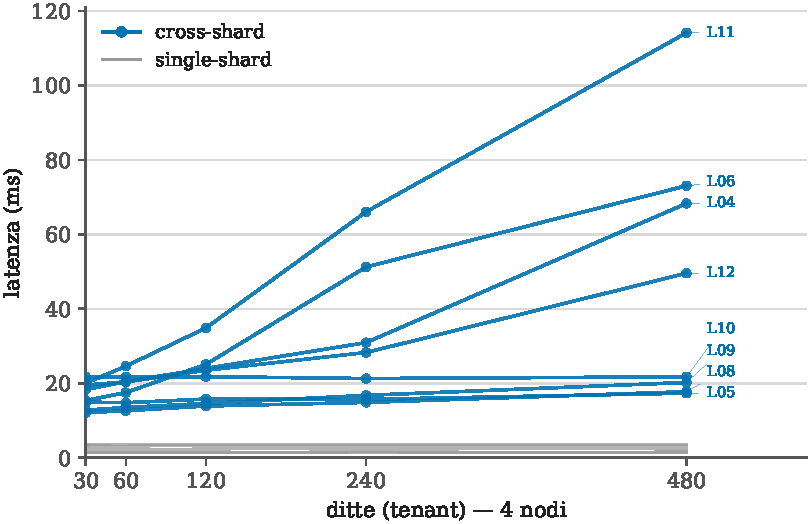
\includegraphics[width=\linewidth]{fig-scaling-dati-citus}
    \end{column}
  \end{columns}
\end{frame}

% ===== Scalabilità per dati: MongoDB =======================================
\begin{frame}{Scalabilità sui dati: MongoDB}
  \begin{columns}[c]
    \begin{column}{0.5\textwidth}
      \small A 4 shard fissi si è spinto il volume \dato{ben oltre le 480 ditte di Citus}, fino a
      \textbf{2630 ditte} (${\sim}$48.000 dipendenti).
      \begin{itemize}\setlength\itemsep{3pt}
        \item A questa scala, e con la \textbf{range size ridotta} sotto il default, il balancer ha
              \dato{distribuito} su \textbf{tutti e 4 gli shard} (CPU 48--65\% ciascuno).
        \item Le \textbf{cross-shard} crescono col volume (L04 26$\to$185\,ms, L11 34$\to$308); L06 e L12
              arrivano ai \dato{secondi} (${\sim}$2.8 e 4.8\,s).
        \item Le query mirate restano \dato{piatte} (${\sim}$2.6\,ms).
      \end{itemize}
    \end{column}
    \begin{column}{0.5\textwidth}
      \centering
      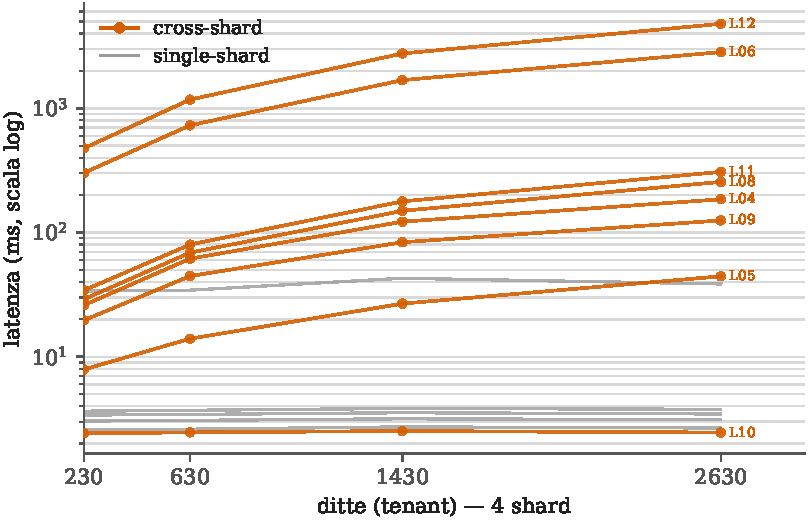
\includegraphics[width=\linewidth]{fig-scaling-dati-mongo}
    \end{column}
  \end{columns}
\end{frame}

% ===== Scalabilità per dati: confronto =====================================
\begin{frame}{Scalabilità sui dati: dove si vedono le differenze}
  \begin{columns}[c]
    \begin{column}{0.47\textwidth}
      \centering
      \begin{tikzpicture}
      \begin{axis}[ybar,ymode=log,width=\linewidth,height=4.9cm,
        symbolic x coords={L04,L06,L11,L12,L13},xtick=data,
        ylabel={latenza (ms, log)},ymin=1,ymax=900,log origin=infty,
        legend style={font=\scriptsize,draw=none,fill=none,at={(0.02,0.98)},anchor=north west},
        bar width=6pt,tick label style={font=\scriptsize},label style={font=\scriptsize},
        ymajorgrids,major grid style={grigiochiaro},enlarge x limits=0.12]
        \addplot[fill=pgblu,draw=pgblu] coordinates {(L04,31)(L06,51)(L11,66)(L12,28)(L13,3.6)};
        \addplot[fill=mongoverde,draw=mongoverde] coordinates {(L04,26)(L06,302)(L11,34)(L12,476)(L13,34)};
        \legend{Citus, MongoDB}
      \end{axis}
      \end{tikzpicture}\\
      {\scriptsize\color{grigio}Latenza a pari scala (${\sim}$230--240 ditte, 4 nodi)}
    \end{column}
    \begin{column}{0.53\textwidth}
      \footnotesize
      \renewcommand{\arraystretch}{1.2}
      \begin{tabular}{@{}lrrl@{}}
        \toprule
        \textbf{Query (ms)} & \textbf{Citus} & \textbf{Mongo} & \\
        \midrule
        L06 assenteismo    & \dato{51}  & 302 & \dato{Citus 6$\times$} \\
        L12 ferie residue  & \dato{28}  & 476 & \dato{Citus 17$\times$} \\
        L13 riepilogo ass. & \dato{3.6} & 34  & \dato{Citus 9$\times$} \\
        \midrule
        L04 gender gap     & 31 & 26          & $\approx$ pari \\
        L11 spesa/cat.     & 66 & \textbf{34} & Mongo 2$\times$ \\
        \bottomrule
      \end{tabular}
      \par\vspace{0.3em}
      {\scriptsize Citus domina le query \textbf{multi-entità} (assenze, ratei: \dato{join indicizzati});
      MongoDB vince dove l'\textbf{embedding} serve già l'aggregato.}
    \end{column}
  \end{columns}
\end{frame}

% ===== Scalabilità per dati: tabella completa =============================
\begin{frame}{Scalabilità sui dati: Citus vs MongoDB (latenza, ms)}
  \centering
  \scriptsize
  \setlength{\tabcolsep}{3pt}
  \renewcommand{\arraystretch}{1.05}
  \begin{tabular}{@{}l *{5}{>{\columncolor{pgblu!9}}r} *{4}{>{\columncolor{mongoverde!9}}r} l@{}}
    \toprule
    & \multicolumn{5}{c}{\textcolor{pgblu}{\textbf{Citus}} (ditte)} & \multicolumn{4}{c}{\textcolor{mongoverde}{\textbf{MongoDB}} (ditte)} & \\
    \cmidrule(lr){2-6}\cmidrule(lr){7-10}
    \textbf{Query} & 30 & 60 & 120 & 240 & 480 & 230 & 630 & 1430 & 2630 & \textbf{vince} \\
    \midrule
    L01 cedolino     & 1.5 & 1.5 & 1.5 & 1.4 & 1.6 & 2.6 & 2.6 & 2.7 & 2.7 & \textcolor{pgblu}{Citus} \\
    L02 cedolini ditta & 1.5 & 1.5 & 1.5 & 1.6 & 1.5 & 3.0 & 3.1 & 3.2 & 3.1 & \textcolor{pgblu}{Citus} \\
    L03 costo/centro & 2.3 & 2.3 & 2.4 & 2.4 & 2.4 & 3.4 & 3.4 & 3.5 & 3.5 & \textcolor{grigio}{$\approx$} \\
    L04 gender gap   & 18.3 & 20.4 & 24.0 & 30.9 & 68.3 & 26.0 & 61.6 & 122 & 185 & \textcolor{mongoverde}{Mongo} \\
    L05 top-N        & 14.9 & 14.8 & 15.8 & 15.7 & 17.4 & 7.9 & 14.0 & 26.8 & 44.4 & \textcolor{mongoverde}{Mongo 2$\times$} \\
    L06 assenteismo  & 15.4 & 17.5 & 25.1 & 51.2 & 73.1 & 302 & 729 & 1685 & 2834 & \textcolor{pgblu}{\textbf{Citus 6$\times$}} \\
    L07 straordinari & 3.2 & 3.2 & 3.2 & 3.2 & 3.3 & 3.6 & 3.7 & 3.8 & 3.8 & \textcolor{grigio}{$\approx$} \\
    L08 trend costo  & 12.1 & 12.6 & 13.9 & 14.9 & 17.8 & 29.0 & 68.8 & 149 & 255 & \textcolor{pgblu}{Citus 2$\times$} \\
    L09 organico     & 12.8 & 13.5 & 14.6 & 16.8 & 20.2 & 19.7 & 44.6 & 83.6 & 125 & \textcolor{grigio}{$\approx$} \\
    L10 ced.\ completo & 21.7 & 21.7 & 21.8 & 21.3 & 21.7 & 2.4 & 2.5 & 2.5 & 2.5 & \textcolor{mongoverde}{\textbf{Mongo 9$\times$}} \\
    L11 spesa/cat.   & 20.1 & 24.6 & 34.9 & 66.0 & 114.1 & 34.2 & 80.0 & 178 & 308 & \textcolor{mongoverde}{Mongo 2$\times$} \\
    L12 ferie residue & 19.5 & 20.4 & 23.5 & 28.3 & 49.6 & 476 & 1174 & 2760 & 4786 & \textcolor{pgblu}{\textbf{Citus 17$\times$}} \\
    L13 riepilogo    & 3.4 & 3.6 & 3.6 & 3.6 & 3.5 & 33.8 & 34.4 & 42.8 & 38.6 & \textcolor{pgblu}{\textbf{Citus 9$\times$}} \\
    \bottomrule
  \end{tabular}
  \par\vspace{0.2em}
  {\scriptsize \textbf{Vince} = più veloce a pari scala (Citus 240 vs Mongo 230 ditte). Citus domina le
  \textcolor{pgblu}{\textbf{query multi-entità}} (assenze, ratei: L06, L12, L13); MongoDB l'\textcolor{mongoverde}{\textbf{aggregato}}
  (cedolino completo L10) e i percentili/top-N (L04, L05, L11).}
\end{frame}

% ===== Dettaglio metriche: Citus ==========================================
\begin{frame}{Scalabilità sui dati: Citus, tutte le metriche (30--480 ditte)}
  \centering
  \tiny
  \setlength{\tabcolsep}{1.7pt}
  \renewcommand{\arraystretch}{1.2}
  \resizebox{\linewidth}{!}{%
  \begin{tabular}{@{}l ccccc ccccc ccccc ccccc ccccc@{}}
    \toprule
    & \multicolumn{5}{c}{\textbf{latenza (ms)}} & \multicolumn{5}{c}{\textbf{throughput (op/s)}}
    & \multicolumn{5}{c}{\textbf{CPU worker (\%)}} & \multicolumn{5}{c}{\textbf{exec worker (ms)}}
    & \multicolumn{5}{c}{\textbf{righe/worker}} \\
    \cmidrule(lr){2-6}\cmidrule(lr){7-11}\cmidrule(lr){12-16}\cmidrule(lr){17-21}\cmidrule(lr){22-26}
    \textbf{Query} & 30&60&120&240&480 & 30&60&120&240&480 & 30&60&120&240&480 & 30&60&120&240&480 & 30&60&120&240&480 \\
    \midrule
    L01 cedolino & 1.5 & 1.5 & 1.5 & 1.4 & 1.6 & 688 & 659 & 655 & 705 & 643 & 3 & 6 & 6 & 5 & 4 & 34 & 36 & 36 & 38 & 34 & 1718 & 1647 & 1636 & 1762 & 1607 \\
    L02 ced.\ ditta & 1.5 & 1.5 & 1.5 & 1.6 & 1.5 & 654 & 659 & 674 & 635 & 682 & 4 & 5 & 4 & 4 & 4 & 43 & 44 & 45 & 33 & 36 & 1636 & 1648 & 1684 & 1588 & 1706 \\
    L03 costo/centro & 2.3 & 2.3 & 2.4 & 2.4 & 2.4 & 433 & 438 & 424 & 414 & 423 & 7 & 7 & 7 & 8 & 8 & 161 & 164 & 171 & 175 & 185 & 51988 & 52548 & 50820 & 49680 & 50748 \\
    L04 gender gap & 18.3 & 20.4 & 24.0 & 30.9 & 68.3 & 55 & 49 & 42 & 32 & 15 & 24 & 26 & 26 & 28 & 38 & 347 & 623 & 947 & 1430 & 1325 & 75667 & 164762 & 283664 & 454734 & 411049 \\
    L05 top-N & 14.9 & 14.8 & 15.8 & 15.7 & 17.4 & 67 & 68 & 63 & 64 & 58 & 20 & 22 & 23 & 27 & 30 & 266 & 423 & 587 & 953 & 1475 & 60240 & 89401 & 98425 & 102080 & 92320 \\
    L06 assenteismo & 15.4 & 17.5 & 25.1 & 51.2 & 73.1 & 65 & 57 & 40 & 20 & 14 & 17 & 32 & 39 & 68 & 91 & 923 & 2445 & 3337 & 3655 & 5274 & 187125 & 326326 & 262342 & 134554 & 94256 \\
    L07 straordinari & 3.2 & 3.2 & 3.2 & 3.2 & 3.3 & 317 & 317 & 309 & 312 & 307 & 11 & 11 & 11 & 11 & 12 & 441 & 478 & 474 & 483 & 480 & 3165 & 3173 & 3093 & 3122 & 3068 \\
    L08 trend costo & 12.1 & 12.6 & 13.9 & 14.9 & 17.8 & 82 & 79 & 72 & 67 & 56 & 12 & 14 & 18 & 27 & 39 & 351 & 673 & 1148 & 2091 & 3460 & 49500 & 68904 & 66960 & 64608 & 54144 \\
    L09 organico & 12.8 & 13.5 & 14.6 & 16.8 & 20.2 & 78 & 74 & 69 & 60 & 49 & 13 & 13 & 14 & 15 & 17 & 125 & 210 & 336 & 546 & 881 & 58234 & 104710 & 185220 & 321186 & 535095 \\
    L10 ced.\ compl. & 21.7 & 21.7 & 21.8 & 21.3 & 21.7 & 46 & 46 & 46 & 47 & 46 & 31 & 32 & 31 & 31 & 30 & 112 & 115 & 115 & 119 & 116 & 115 & 115 & 115 & 118 & 115 \\
    L11 spesa/cat. & 20.1 & 24.6 & 34.9 & 66.0 & 114.1 & 50 & 41 & 29 & 15 & 9 & 25 & 27 & 29 & 42 & 52 & 543 & 1102 & 1292 & 1404 & 1718 & 69158 & 136854 & 195912 & 213332 & 246070 \\
    L12 ferie res. & 19.5 & 20.4 & 23.5 & 28.3 & 49.6 & 51 & 49 & 43 & 35 & 20 & 30 & 35 & 38 & 44 & 65 & 528 & 1007 & 1576 & 2569 & 3100 & 3842 & 7365 & 12780 & 21240 & 24240 \\
    L13 riepilogo & 3.4 & 3.6 & 3.6 & 3.6 & 3.5 & 291 & 279 & 276 & 280 & 289 & 10 & 10 & 10 & 10 & 10 & 230 & 233 & 224 & 228 & 193 & 7281 & 6978 & 6895 & 7010 & 7220 \\
    \bottomrule
  \end{tabular}}
  \par\vspace{0.2em}
  {\scriptsize \texttt{blk\_read}${=}0$ (dati in RAM): il degrado è CPU-bound. Sulle cross-shard le righe scandite
  per worker crescono col volume e il throughput cala; le single-shard restano costanti.}
\end{frame}

% ===== Dettaglio metriche: MongoDB =========================================
\begin{frame}{Scalabilità sui dati: MongoDB, tutte le metriche}
  \centering
  \scriptsize
  \setlength{\tabcolsep}{4pt}
  \renewcommand{\arraystretch}{1.0}
  \begin{tabular}{@{}l rrrr rrrr rrrr@{}}
    \toprule
    & \multicolumn{4}{c}{\textbf{latenza (ms)}} & \multicolumn{4}{c}{\textbf{throughput (op/s)}}
    & \multicolumn{4}{c}{\textbf{CPU media/shard (\%)}} \\
    \cmidrule(lr){2-5}\cmidrule(lr){6-9}\cmidrule(lr){10-13}
    \textbf{Query} & 230 & 630 & 1430 & 2630 & 230 & 630 & 1430 & 2630 & 230 & 630 & 1430 & 2630 \\
    \midrule
    L01 cedolino      & 2.6 & 2.6 & 2.7 & 2.7 & 385 & 383 & 367 & 374 & 6 & 5 & 5 & 6 \\
    L02 cedolini ditta& 3.0 & 3.1 & 3.2 & 3.1 & 329 & 325 & 316 & 321 & 6 & 6 & 6 & 6 \\
    L03 costo/centro  & 3.4 & 3.4 & 3.5 & 3.5 & 294 & 291 & 282 & 289 & 6 & 7 & 6 & 6 \\
    L04 gender gap    & 26.0 & 61.6 & 122 & 185 & 38 & 16 & 8 & 5 & 14 & 15 & 18 & 22 \\
    L05 top-N         & 7.9 & 14.0 & 26.8 & 44.4 & 127 & 72 & 37 & 22 & 31 & 43 & 54 & 58 \\
    L06 assenteismo   & 302 & 729 & 1685 & 2834 & 3 & 1 & 1 & 0 & 59 & 66 & 70 & 75 \\
    L07 straordinari  & 3.6 & 3.7 & 3.8 & 3.8 & 274 & 270 & 261 & 265 & 8 & 8 & 8 & 8 \\
    L08 trend costo   & 29.0 & 68.8 & 149 & 256 & 34 & 14 & 7 & 4 & 49 & 58 & 64 & 69 \\
    L09 organico      & 19.7 & 44.6 & 83.6 & 125 & 51 & 22 & 12 & 8 & 14 & 16 & 20 & 23 \\
    L10 ced.\ completo& 2.4 & 2.5 & 2.5 & 2.5 & 413 & 406 & 396 & 407 & 4 & 3 & 3 & 3 \\
    L11 spesa/cat.    & 34.2 & 80.0 & 178 & 308 & 29 & 12 & 6 & 3 & 48 & 56 & 61 & 65 \\
    L12 ferie residue & 476 & 1174 & 2760 & 4786 & 2 & 1 & 0 & 0 & 57 & 62 & 68 & 89 \\
    L13 riepilogo     & 33.8 & 34.4 & 42.8 & 38.6 & 30 & 29 & 23 & 26 & 17 & 17 & 17 & 21 \\
    \bottomrule
  \end{tabular}
  \par
  {\scriptsize Disco letto ${\approx}0$ (dati in RAM). Le cross-shard (L06, L12) \dato{saturano la CPU su tutti
  gli shard} e crollano nel throughput; le mirate (L01, L10) restano ${\sim}$400 op/s.}
\end{frame}

% ===== 8. Confronto letture / analitica =====================================
\section{Confronto}
\begin{frame}{Confronto nelle letture: comportamento e idoneità}
  \begin{columns}[T]
    \begin{column}{0.5\textwidth}
      \begin{sysblock}{pgblu}{PostgreSQL + Citus}
        \footnotesize
        \textbf{Sui nodi:} \textcolor{pgblu}{\textbf{scala}} --- col rebalance esplicito le analitiche cross-shard migliorano ${\sim}4\times$ da 1 a 4 nodi.
        \par\smallskip
        \textbf{Sui dati:} degrada col volume (il degrado \emph{accelera}), ma le query mirate restano costanti.
        \par\smallskip
        \textbf{Più adatto a:} analitiche \textcolor{pgblu}{\textbf{multi-entità}} --- assenze L06 (6$\times$), ferie/ratei L12 (17$\times$), riepiloghi L13 (9$\times$): \emph{join} indicizzati.
      \end{sysblock}
    \end{column}
    \begin{column}{0.5\textwidth}
      \begin{sysblock}{mongoverde}{MongoDB}
        \footnotesize
        \textbf{Sui nodi:} col dataset piccolo del test \textcolor{mongoverde}{\textbf{non ridistribuisce}}; più veloce in assoluto.
        \par\smallskip
        \textbf{Sui dati:} a volume grande distribuisce (chunk ridotti, fino a 2630 ditte); scandire gli \textbf{array annidati} (L06, L12) porta ai \emph{secondi}.
        \par\smallskip
        \textbf{Più adatto a:} informazioni \textcolor{mongoverde}{\textbf{aggregate}} --- cedolino completo L10 (9$\times$, un solo \texttt{findOne}) e aggregati/percentili semplici (L04, L05, L11).
      \end{sysblock}
    \end{column}
  \end{columns}
  \begin{keyblock}{In sintesi --- caso d'uso HR}
    \footnotesize Nessuno dei due prevale in assoluto: l'idoneità \textbf{dipende dal tipo di query}. 
    Per il \textbf{reporting analitico multi-entità} \textcolor{pgblu}{\textbf{Citus risulta più efficiente e scala aggiungendo nodi}}; per le \textbf{letture del singolo cedolino} (l'aggregato) \textcolor{mongoverde}{\textbf{MongoDB è più rapido}}.
  \end{keyblock}
\end{frame}

% ===== 9a. Scritture: Citus ================================================
\begin{frame}{Scritture: PostgreSQL + Citus}
  \begin{columns}[c]
    \begin{column}{0.5\textwidth}
      \small
      \begin{itemize}\setlength\itemsep{5pt}
        \item \textbf{Co-locazione}: ogni scrittura di un tenant colpisce \dato{un solo nodo}.
        \item Il costo cresce con la \textbf{complessità transazionale}: dall'\texttt{UPDATE} di 1 riga
              (U02, 1.7\,ms) alla \textbf{transazione multi-tabella} I03 (57\,ms) --- fattore ${\sim}35\times$.
        \item L'unica che tocca \textbf{tutti i nodi} è U03 (reference table replicata): 21\,ms, ma resta contenuta.
      \end{itemize}
    \end{column}
    \begin{column}{0.5\textwidth}
      \centering
      \begin{tikzpicture}
      \begin{axis}[ybar,ymode=log,width=\linewidth,height=5cm,
        symbolic x coords={U02,U01,U04,I01,U03,I03},xtick=data,
        ylabel={latenza (ms, log)},ymin=1,ymax=120,
        bar width=10pt,tick label style={font=\scriptsize},label style={font=\scriptsize},
        ymajorgrids,major grid style={grigiochiaro},enlarge x limits=0.12]
        \addplot[fill=pgblu,draw=pgblu] coordinates {(U02,1.7)(U01,3.7)(U04,3.8)(I01,10.6)(U03,21.1)(I03,57.4)};
      \end{axis}
      \end{tikzpicture}\\
      {\scriptsize\color{grigio}Latenza per operazione (4 nodi, $N{=}300$, tenant fisso)}
    \end{column}
  \end{columns}
\end{frame}

% ===== 9b. Scritture: MongoDB ==============================================
\begin{frame}{Scritture: MongoDB}
  \begin{columns}[c]
    \begin{column}{0.5\textwidth}
      \small
      \begin{itemize}\setlength\itemsep{5pt}
        \item Inserire un \textbf{cedolino} (I03) è \dato{economico}: 11\,ms, \textbf{un solo documento},
              niente transazione multi-tabella.
        \item Le scritture singole sono veloci (${\sim}$3.6\,ms).
        \item \textbf{Ma} aggiornare un \textbf{dato condiviso} (U03) costa \dato{356\,ms}: lo snapshot
              denormalizzato va riscritto in \textbf{ogni cedolino} $\Rightarrow$ CPU ${\sim}95\%$, 265\,MB scritti.
      \end{itemize}
    \end{column}
    \begin{column}{0.5\textwidth}
      \centering
      \begin{tikzpicture}
      \begin{axis}[ybar,ymode=log,width=\linewidth,height=5cm,
        symbolic x coords={U01,U02,U04,I01,I03,U03},xtick=data,
        ylabel={latenza (ms, log)},ymin=1,ymax=700,
        bar width=10pt,tick label style={font=\scriptsize},label style={font=\scriptsize},
        ymajorgrids,major grid style={grigiochiaro},enlarge x limits=0.12]
        \addplot[fill=mongoverde,draw=mongoverde] coordinates {(U01,3.6)(U02,3.6)(U04,3.6)(I01,8.6)(I03,11.1)(U03,355.9)};
      \end{axis}
      \end{tikzpicture}\\
      {\scriptsize\color{grigio}U03 esplode: \emph{write amplification} sull'embedding}
    \end{column}
  \end{columns}
\end{frame}

% ===== 9c. Scritture: confronto ============================================
\begin{frame}{Scritture: confronto Citus vs MongoDB}
  \begin{columns}[c]
    \begin{column}{0.52\textwidth}
      \centering
      \begin{tikzpicture}
      \begin{axis}[ybar,ymode=log,width=\linewidth,height=5cm,
        symbolic x coords={U01,U02,U04,I01,I03,U03},xtick=data,
        ylabel={latenza (ms, log)},ymin=1,ymax=800,
        legend style={font=\scriptsize,at={(0.02,0.98)},anchor=north west,draw=none,fill=none},
        bar width=6pt,tick label style={font=\scriptsize},label style={font=\scriptsize},
        ymajorgrids,major grid style={grigiochiaro},enlarge x limits=0.1]
        \addplot[fill=pgblu,draw=pgblu] coordinates {(U01,3.7)(U02,1.7)(U04,3.8)(I01,10.6)(I03,57.4)(U03,21.1)};
        \addplot[fill=mongoverde,draw=mongoverde] coordinates {(U01,3.6)(U02,3.6)(U04,3.6)(I01,8.6)(I03,11.1)(U03,355.9)};
        \legend{Citus,MongoDB}
      \end{axis}
      \end{tikzpicture}
    \end{column}
    \begin{column}{0.48\textwidth}
      \footnotesize
      \textbf{I03} cedolino: \textcolor{mongoverde}{\textbf{Mongo 5$\times$}} --- 1 documento vs transazione
      su 7 tabelle.\par\smallskip
      \textbf{U03} dato condiviso: \textcolor{pgblu}{\textbf{Citus 17$\times$}} --- 1 riga normalizzata vs
      snapshot in ogni cedolino.\par\smallskip
      Le altre scritture: \dato{sostanzialmente pari}.
      \par\smallskip
      \textbf{Scalabilità} (entrambi): ogni scrittura \dato{co-loca su un nodo} --- aggiungere nodi non abbassa
      la singola scrittura, ma il \textbf{throughput} cresce con i tenant in parallelo.
      \par\medskip
      \begin{keyblock}{In sintesi}
        \footnotesize L'\textbf{embedding} rende economico \emph{scrivere l'aggregato} ma costoso
        \emph{propagare una modifica condivisa}; la \textbf{normalizzazione} fa l'opposto.
      \end{keyblock}
    \end{column}
  \end{columns}
\end{frame}

% ===== 9d. Guasti: Citus ===================================================
\begin{frame}{Guasti: PostgreSQL + Citus}
  \begin{columns}[c]
    \begin{column}{0.5\textwidth}
      \small
      \textbf{Test}: L04 in loop per 45\,s, un worker spento tra 10 e 25\,s.
      \begin{itemize}\setlength\itemsep{4pt}
        \item Col nodo del tenant giù la query \dato{fallisce all'istante} (\textbf{fail-fast}, connection refused).
        \item \textbf{righe $\to$ 0}: nessun risultato parziale (\textbf{CP}).
        \item Tanti errori \enquote{brevi} (${\sim}$70\,ms) $\Rightarrow$ error-rate \dato{alto ($\sim$51\%)}.
        \item Recupero \dato{automatico} al ritorno del nodo (${\sim}$0.5\,s).
      \end{itemize}
    \end{column}
    \begin{column}{0.5\textwidth}
      \centering
      \begin{tikzpicture}
      \begin{axis}[width=\linewidth,height=4.8cm,xlabel={tempo (s)},ylabel={latenza (ms)},
        xmin=0,xmax=45,ymin=0,ymax=220,tick label style={font=\scriptsize},label style={font=\scriptsize},
        ymajorgrids,major grid style={grigiochiaro}]
        \fill[red!10] (axis cs:10.5,0) rectangle (axis cs:25.5,220);
        \node[font=\tiny,red!60!black] at (axis cs:18,205) {nodo gi\`u};
        \addplot[pgblu,very thick] coordinates {(0,147)(5,157)(8,177)(10,168)(10.6,71)(14,85)(18,73)(22,71)(25,74)(25.6,154)(30,164)(37,166)(44,150)};
      \end{axis}
      \end{tikzpicture}\\
      {\scriptsize\color{grigio}Fallimento \dato{immediato}: la latenza \emph{cala} (errori istantanei)}
    \end{column}
  \end{columns}
\end{frame}

% ===== 9e. Guasti: MongoDB =================================================
\begin{frame}{Guasti: MongoDB}
  \begin{columns}[c]
    \begin{column}{0.5\textwidth}
      \small
      \textbf{Test}: stesso protocollo, shard con i dati spento tra 10 e 25\,s.
      \begin{itemize}\setlength\itemsep{4pt}
        \item Con lo shard giù la query si \dato{blocca fino al timeout} (${\sim}$5\,s per operazione).
        \item \textbf{righe $\to$ 0}: nessun risultato parziale (\textbf{CP}).
        \item Pochi errori \enquote{lunghi} $\Rightarrow$ error-rate \dato{basso ($\sim$7\%)}, ma ognuno costa 5\,s.
        \item Recupero \dato{automatico} al ritorno dello shard (${\sim}$0.25\,s).
      \end{itemize}
    \end{column}
    \begin{column}{0.5\textwidth}
      \centering
      \begin{tikzpicture}
      \begin{axis}[width=\linewidth,height=4.8cm,xlabel={tempo (s)},ylabel={latenza (ms, log)},
        ymode=log,xmin=0,xmax=45,ymin=300,ymax=8000,
        tick label style={font=\scriptsize},label style={font=\scriptsize},
        ymajorgrids,major grid style={grigiochiaro}]
        \fill[red!10] (axis cs:10.5,300) rectangle (axis cs:25.5,8000);
        \node[font=\tiny,red!60!black] at (axis cs:18,6500) {shard gi\`u};
        \addplot[mongoverde,very thick] coordinates {(0,697)(6,689)(9,693)(10.6,5005)(18,5005)(25,5000)(25.6,700)(31,707)(38,696)(43,699)};
      \end{axis}
      \end{tikzpicture}\\
      {\scriptsize\color{grigio}Blocco: la latenza \dato{sale a ${\sim}$5\,s} (timeout per operazione)}
    \end{column}
  \end{columns}
\end{frame}

% ===== 9f. Guasti: confronto ===============================================
\begin{frame}{Guasti: confronto Citus vs MongoDB}
  \begin{columns}[c]
    \begin{column}{0.54\textwidth}
      \centering
      \begin{tikzpicture}
      \begin{axis}[width=\linewidth,height=5cm,xlabel={tempo (s)},ylabel={latenza (ms, log)},
        ymode=log,xmin=0,xmax=45,ymin=40,ymax=8000,
        legend style={font=\scriptsize,at={(0.98,0.5)},anchor=east,draw=none,fill=white,fill opacity=0.75},
        tick label style={font=\scriptsize},label style={font=\scriptsize},
        ymajorgrids,major grid style={grigiochiaro}]
        \fill[red!10] (axis cs:10.5,40) rectangle (axis cs:25.5,8000);
        \node[font=\tiny,red!60!black] at (axis cs:18,6200) {nodo gi\`u};
        \addplot[pgblu,very thick] coordinates {(0,150)(8,170)(10,165)(10.6,71)(18,73)(25,74)(25.6,158)(35,162)(45,152)};
        \addplot[mongoverde,very thick] coordinates {(0,695)(9,693)(10.6,5005)(18,5005)(25,5000)(25.6,700)(35,702)(45,698)};
        \legend{Citus,MongoDB}
      \end{axis}
      \end{tikzpicture}\\
      {\scriptsize\color{grigio}Durante il down, per \textbf{entrambi} \emph{righe $\to$ 0} (nessun parziale)}
    \end{column}
    \begin{column}{0.46\textwidth}
      \footnotesize
      \textbf{Elementi comuni} (entrambi \textbf{CP}): indisponibilità reale \dato{${\sim}15$\,s}, assenza di
      risultati parziali (righe $=0$), ripristino automatico.
      \par\smallskip
      \textbf{Modalità di fallimento differente}: \textcolor{pgblu}{\textbf{Citus}} rifiuta la connessione
      all'istante (${\sim}70$\,ms per tentativo); \textcolor{mongoverde}{\textbf{MongoDB}} attende la scadenza
      del timeout (${\sim}5$\,s per operazione).
      \par\medskip
      \begin{keyblock}{Lettura dell'error-rate}
        \footnotesize Il valore grezzo (51\% contro 7\%) non è confrontabile: dipende dalla \textbf{durata di
        ogni tentativo fallito}, non dalla gravità del guasto. I fallimenti \emph{fail-fast}, istantanei, si
        ripetono molte più volte nella stessa finestra; il riferimento corretto è l'\textbf{indisponibilità
        reale}, identica per entrambi.
      \end{keyblock}
    \end{column}
  \end{columns}
\end{frame}

% ===== 9g. Evoluzione dello schema =========================================
\begin{frame}{Evoluzione dello schema in corso d'opera}
  \small Scenario: aggiungere \textbf{turni e ferie} a un sistema \textbf{già popolato}.
  \vspace{0.3em}
  \begin{center}
  \scriptsize
  \renewcommand{\arraystretch}{1.1}
  \begin{tabular}{@{}p{0.19\linewidth} p{0.36\linewidth} p{0.36\linewidth}@{}}
    \toprule
    & \textcolor{pgblu}{\textbf{PostgreSQL + Citus}} \newline \textcolor{pgblu}{\footnotesize schema esplicito}
    & \textcolor{mongoverde}{\textbf{MongoDB}} \newline \textcolor{mongoverde}{\footnotesize schema flessibile} \\
    \midrule
    \textbf{Come si applica} & \texttt{ALTER TABLE} o nuova tabella distribuita, co-locata su \texttt{tenant\_id}
      & Si scrivono i nuovi campi/array solo nei documenti nuovi \\
    \textbf{Dati esistenti} & \dato{Backfill} e propagazione a \textbf{tutti gli shard}
      & \dato{Intatti}: documenti vecchi e nuovi coesistono \\
    \textbf{Governo} & Vincoli e integrità \textbf{garantiti dal DBMS}
      & Demandato all'applicazione (\emph{schema-on-read}) \\
    \textbf{Costo / rischio} & Migrazione transazionale, possibili \textbf{lock}
      & Estensione \textbf{quasi immediata} \\
    \bottomrule
  \end{tabular}
  \end{center}
  \vspace{0.2em}
  \begin{keyblock}{In sintesi}
    \footnotesize Il \textbf{documentale} privilegia l'\textcolor{mongoverde}{\textbf{agilità evolutiva}} (i dati
    esistenti non si toccano); il \textbf{relazionale} le \textcolor{pgblu}{\textbf{garanzie di integrità}} durante
    il cambiamento.
  \end{keyblock}
\end{frame}

% ===== 10. Conclusioni ======================================================
\section{Conclusioni}
\begin{frame}{Conclusioni}
  Gli esperimenti \dato{confermano l'ipotesi iniziale}: in \textbf{lettura e scrittura}, le operazioni su
  \textcolor{pgblu}{\textbf{più entità}} sono più efficienti sul modello \textbf{relazionale} (Citus: L06, L12,
  L13, U03), quelle sull'\textcolor{mongoverde}{\textbf{aggregato o singola entità}} sul \textbf{non relazionale}
  (MongoDB: L10, I03).
  \par\smallskip Sulla \textbf{scalabilità in ambiente distribuito} i due sistemi seguono approcci distinti:
  \par\smallskip
  \begin{columns}[T]
    \begin{column}{0.5\textwidth}
      \begin{sysblock}{pgblu}{PostgreSQL + Citus}
        \footnotesize Distribuzione \dato{esplicita} (rebalance on-demand), a qualsiasi volume: aggiungendo
        nodi le analitiche migliorano \dato{$3.8$--$4.6\times$} (1$\to$4 nodi).
      \end{sysblock}
    \end{column}
    \begin{column}{0.5\textwidth}
      \begin{sysblock}{mongoverde}{MongoDB}
        \footnotesize Distribuzione \dato{automatica, legata al volume}: col dataset piccolo del test resta su
        un solo shard; \dato{a volume pieno} distribuisce su tutti gli shard.
      \end{sysblock}
    \end{column}
  \end{columns}
  \smallskip
  \begin{keyblock}{In sintesi}
    \footnotesize \textcolor{pgblu}{\textbf{Citus}} ridistribuisce su richiesta, con guadagno immediato a
    qualsiasi volume (${\sim}4\times$); \textcolor{mongoverde}{\textbf{MongoDB}} usa un balancer automatico, che
    interviene solo oltre una soglia di dati (raggiunta col dataset finale, non con quello iniziale).
  \end{keyblock}
\end{frame}

\end{document}
